\documentclass[../eva1_scion.tex]{subfiles}
\begin{document}
    \chapter{Results}
    \section{Isolation Domains}
    SCION borrows basic ideas from the Border Gateway Protocol (BGP) like the idea of an Autonomous System (AS) which, like in BGP, repesents the smalest organisational unit. However, SCION introduces an additonal organisational unit called the Isolation Domain (ISD). The structure of an indivual ISD is ilustrated in \ref{fig:isd}a. An ISD is comprised of multiple core ASes, form logical unit whos members share a common set of resources and mutualy trust each other. As their name states, ISDs are intended to be selfsuficient units, the internal state of which must not leak out into other ISDs. \cite{scion_2011} While an arbitrary AS can be a member of an arbitrary ISD, or even multiple ISDs, it is expected that ISDs will form along shared comercial interests, legal juristiction or other political borders. \cite{scion_2017}.

    \subsection{IDS structure}
    As shown in ilustration \ref{fig:isd}a the main structure of an IDS is an undirected graph formed by a set of core ASes in the ISD core, client ASes and biderectional links between individual ASes. ASes may be connected by multiple redundant links. Although a link always carries biderctional traffic, there is an implied top down hirarchy of providers and consumers between the tiers in the graph. As in BGP a pair of ASes may enter an peering agreement, which is ilustrated is a dashed line. Links are also called path segments.

    \subsection{AS and ISD Componants}
    In the following we will explore the componantes which are required to run an SCION AS and by extension a ISD since a single core AS is sufficient to form an IDS.

    SCION ASes look similar too their BGP cousins so fare as that they have internal routers and border routers and a set of routes through the AS. These ensure connectivity inside the AS and to neighbouring ASes. Border routers must be SCION enabled and must addhere to the common rules agreed upon inside the ISD, however each AS is free to choos its internal structure. In addition each AS needs at least a beacon server, a certificate server and a path server. Beacon servers are responbsible for path discovery and are required for beaconing process described in section \ref{ssec:beaconing}. Path server are repsonsible for caching and disimination of path information. They are involved in path resolution and assembly discussed in section \ref{ssec:path_assembly}. As SCION makes extensive us of certificates to validate paths and intities, certificate servers are deployed to cache and provide certificates in an AS.
    
    A core AS differs from other ASes in serveral important aspects. First of all core ASes have border routers which are connected to cores ASes in neighbouring. The beacon servers in the core ASes also take part in inter IDS beaconing (see section \ref{ssec:beaconing}), thus their path servers also hold path information on how to reach neighbouring ASes. Further more the ISD core is responsible for maintaining the trust root configuration (TRC).

    The trust root configuration (TRC) is policy which governs the operations of an ISD. The TRC lists the trust roots used in an ISD and thus is the central anchor of trust in an IDS. It is negotiated between the members of the ISD core and all ASes whishing to join  an ISD need to accept the TRC. Neighbouring ISDs acknowledge an ISDs TRC by signing it. This makes ASes communicting across ISD bordes able to trust signatures originating from an neighouring ISD. 

    \begin{figure}[h]
        \centering
        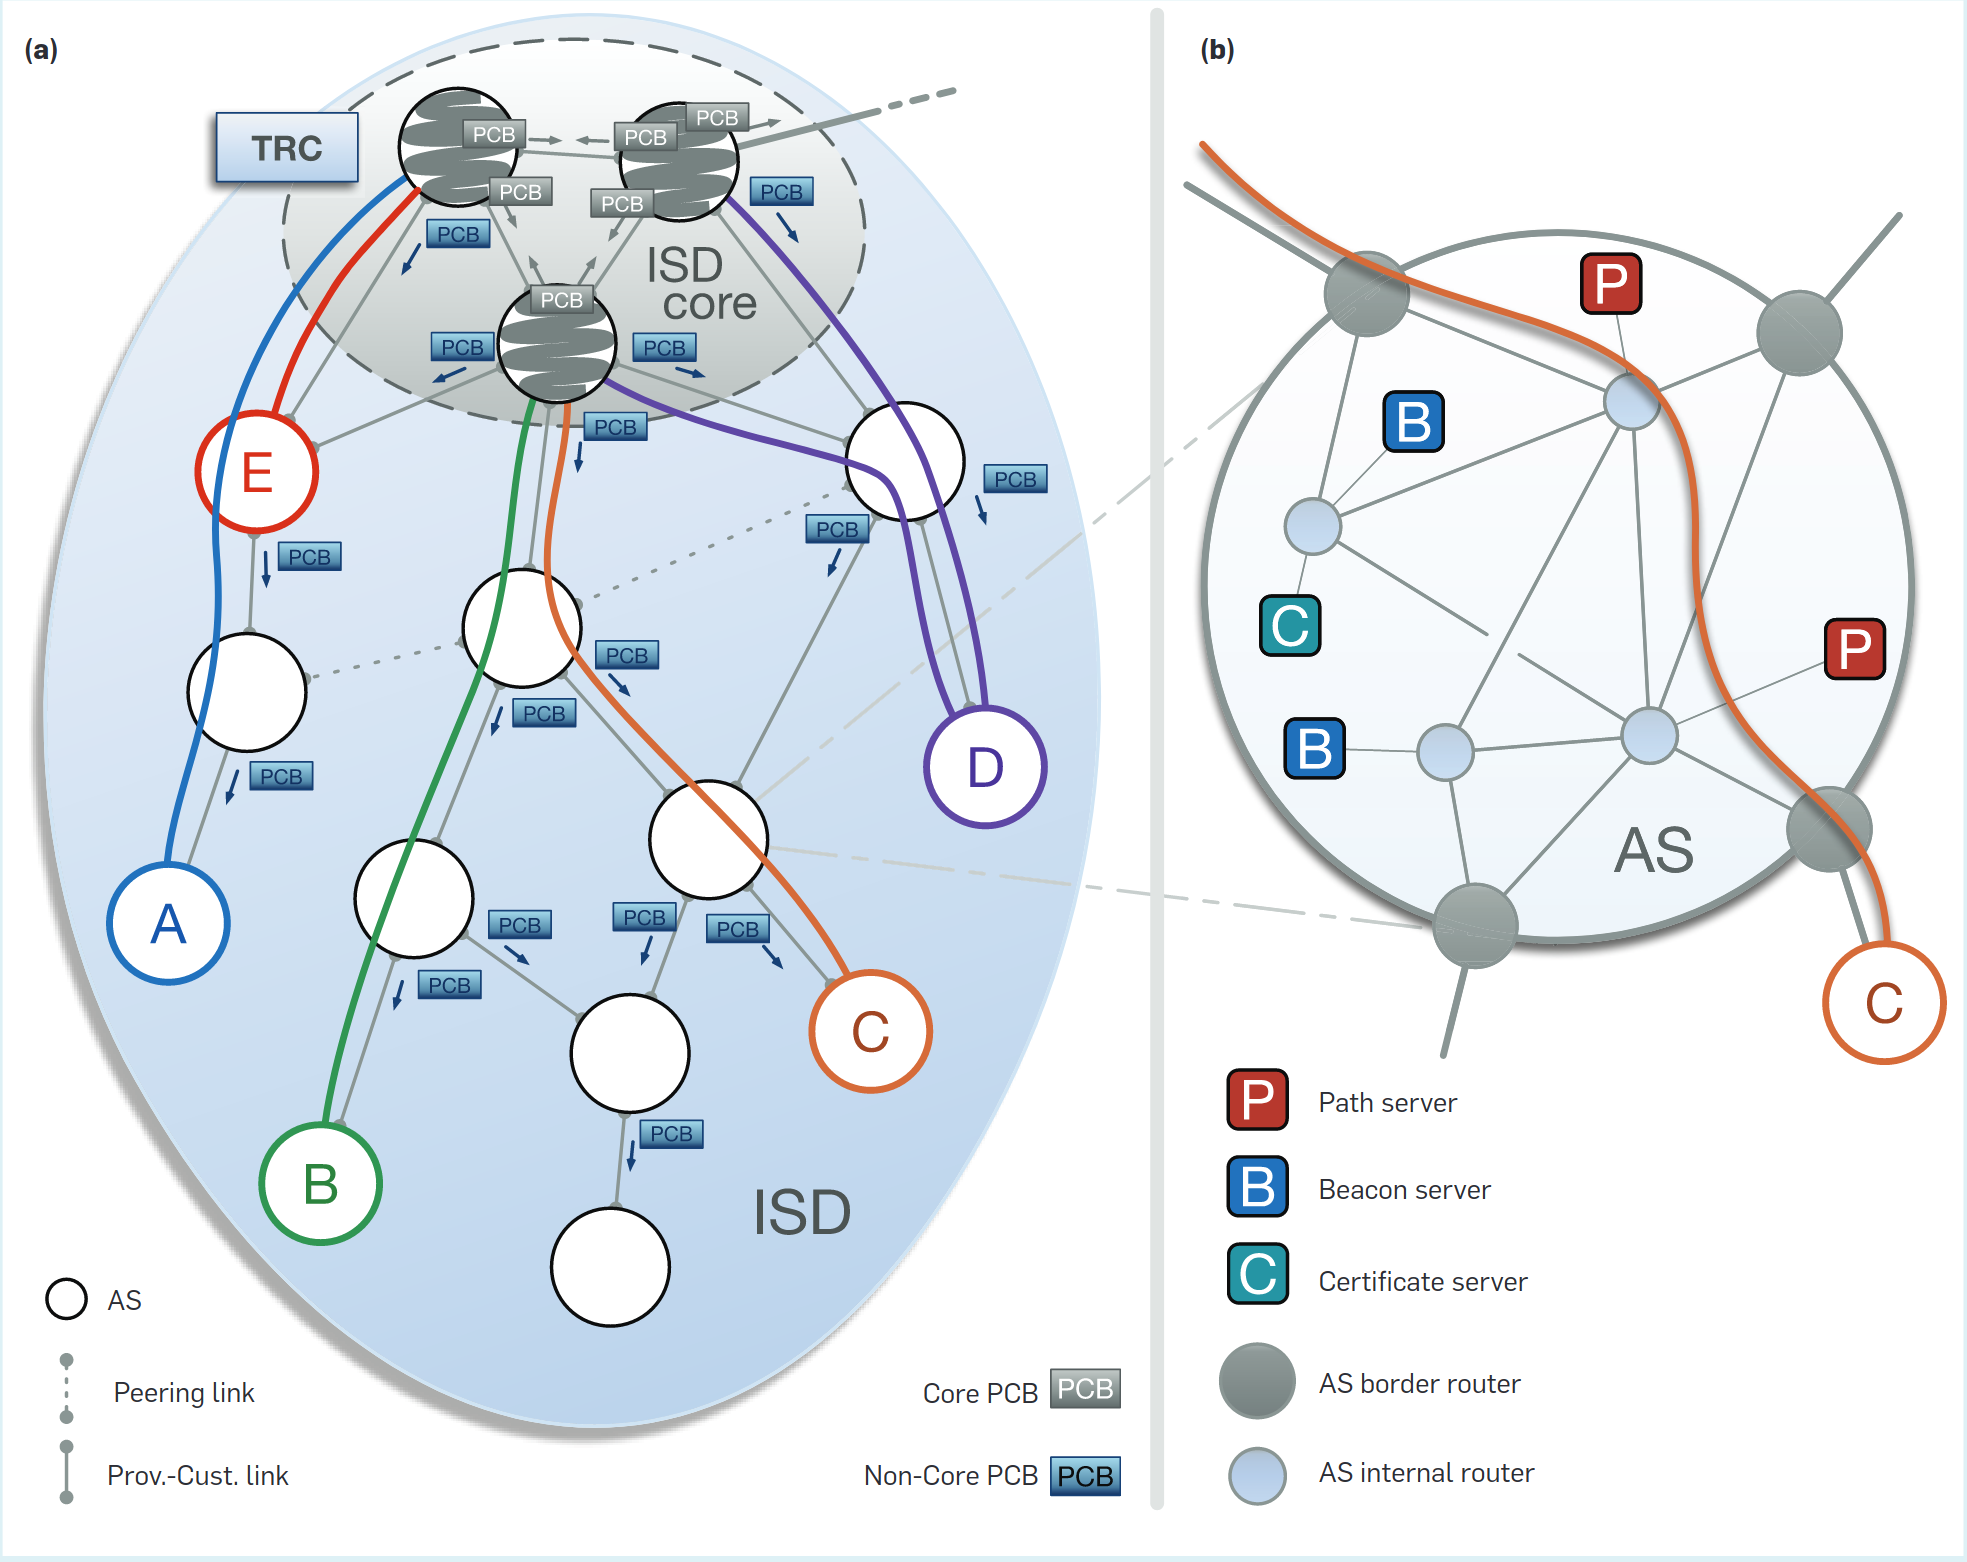
\includegraphics[width=0.8\linewidth]{scion_isd.png}
        \caption{Internal structure of an ISD. From \cite{scion_2017}}%
        \label{fig:isd}
    \end{figure}

    Until now we looked at the static componants which make up an ISD, however the real world internet is not a static thing, so an ISD isn't either. To better manage complexity SCION is devided into a controll plane and a data plane. The control plane is concerned with discovering and maintaining paths, while the data plane uses these paths in the processes of path assembly and packet fowarding.

    \section{Control Plane}
    As mentioned above SCION has taken inspiration form BGP and the paths discovery is an other place where this is evident. SCION uses an beaconing process to discover all available paths and disiminate certain information inside an ISDs.  These beacons are called patch-segment construction beacons (PCBS) and are  sent from beacon servers in the ISD core t travle down the ISD graph as an policy constrained multipath flood. \cite{scion_2011}.

    \subsection{Path Discovery by Beaconing}\label{ssec:beaconing}
    Initialy the path server in a core ISD issues a PCB containing only the exit interface it originates from. A path server in a neighbouring AS receiving an incomming will forward it to all its client ASes. Befor forwarding the PCB it creates a crypotgraphically signed record of the ingress inteface, egress interface and available peers and appends it to the PCB. In this way a PCB accumulates path information as a so called path-segment while it is forwarded through the ISD. The information received in PCBs is cached in the local path servers, so end hosts in an ISD have a way to look up path information. Important to note is that PCBs are not sent out through peering links as this would lead douplicate paths or might lead to intra-ISD beacons leaking into other ISDs.

    PCBs traveling down collect what are called down paths, but since all paths forward packets bidirectionally, each down-segment can be converted into an up-segment by inverting the order or traversed ASes. Once an AS has received a number of path segments it can register some of them as down-paths segmemts with the core path servers. This has two important consequences:  An AS always knows how to reach its ISD core by creating recoding path segments from PCBs, however for a local path server to optain down-paths to other ASes it needs to query the a path server in the core. This gives each AS the unique ability to control by which paths it would whishes to be reached.

    Selecting down-paths to register with the




    \section{Data Plane}

    \subsection{Path Assembly} \label{ssec:path_assembly}
    \subsection{Data Forwading}
    
    \section{Trust Management}
    \subsection{Trust agility}
    \section{SCION Adoption}


\end{document}
